% -*- coding: utf-8 -*-
%-------------------------designed by zcf--------------
\documentclass[UTF8,a4paper,10pt]{ctexart}
\usepackage[left=3.17cm, right=3.17cm, top=2.74cm, bottom=2.74cm]{geometry}
\usepackage{amsmath}
\usepackage{graphicx,subfig}
\usepackage{float}
\usepackage{subfigure}  
\usepackage{cite}
\usepackage{caption}
\usepackage{enumerate}
\usepackage{booktabs} %表格
\usepackage{multirow}
\newcommand{\tabincell}[2]{\begin{tabular}{@{}#1@{}}#2\end{tabular}}  %表格强制换行
%-------------------------字体--------------
% \usepackage{times} 
\usepackage{ctex}
\setCJKmainfont[ItalicFont=Noto Sans CJK SC Bold, BoldFont=Noto Serif CJK SC Black]{Noto Serif CJK SC}
\newcommand{\yihao}{\fontsize{26pt}{36pt}\selectfont}           % 一号, 1.4 倍行距
\newcommand{\erhao}{\fontsize{22pt}{28pt}\selectfont}          % 二号, 1.25倍行距
\newcommand{\xiaoer}{\fontsize{18pt}{18pt}\selectfont}          % 小二, 单倍行距
\newcommand{\sanhao}{\fontsize{16pt}{24pt}\selectfont}  %三号字
\newcommand{\xiaosan}{\fontsize{15pt}{22pt}\selectfont}        % 小三, 1.5倍行距
\newcommand{\sihao}{\fontsize{14pt}{21pt}\selectfont}            % 四号, 1.5 倍行距
\newcommand{\banxiaosi}{\fontsize{13pt}{19.5pt}\selectfont}    % 半小四, 1.5倍行距
\newcommand{\xiaosi}{\fontsize{12pt}{18pt}\selectfont}            % 小四, 1.5倍行距
\newcommand{\dawuhao}{\fontsize{11pt}{11pt}\selectfont}       % 大五号, 单倍行距
\newcommand{\wuhao}{\fontsize{10.5pt}{15.75pt}\selectfont}    % 五号, 单倍行距
%-------------------------章节名----------------
\usepackage{ctexcap} 
\CTEXsetup[name={,、},number={ \chinese{section}}]{section}
\CTEXsetup[name={(,)},number={\chinese{subsection}}]{subsection}
\CTEXsetup[name={,.},number={\arabic{subsubsection}}]{subsubsection}
%-------------------------页眉页脚--------------
\usepackage{fancyhdr}
\pagestyle{fancy}
\lhead{\kaishu \leftmark}
% \chead{}
\rhead{\kaishu 并行程序设计实验报告}%加粗\bfseries 
\lfoot{}
\cfoot{\thepage}
\rfoot{}
\renewcommand{\headrulewidth}{0.1pt}  
\renewcommand{\footrulewidth}{0pt}%去掉横线
\newcommand{\HRule}{\rule{\linewidth}{0.5mm}}%标题横线
\newcommand{\HRulegrossa}{\rule{\linewidth}{1.2mm}}
%-----------------------伪代码------------------
\usepackage{algorithm}  
\usepackage{algorithmicx}  
\usepackage{algpseudocode}  
\floatname{algorithm}{Algorithm}  
\renewcommand{\algorithmicrequire}{\textbf{Input:}}  
\renewcommand{\algorithmicensure}{\textbf{Output:}} 
\usepackage{lipsum}  
\makeatletter
\newenvironment{breakablealgorithm}
  {% \begin{breakablealgorithm}
  \begin{center}
     \refstepcounter{algorithm}% New algorithm
     \hrule height.8pt depth0pt \kern2pt% \@fs@pre for \@fs@ruled
     \renewcommand{\caption}[2][\relax]{% Make a new \caption
      {\raggedright\textbf{\ALG@name~\thealgorithm} ##2\par}%
      \ifx\relax##1\relax % #1 is \relax
         \addcontentsline{loa}{algorithm}{\protect\numberline{\thealgorithm}##2}%
      \else % #1 is not \relax
         \addcontentsline{loa}{algorithm}{\protect\numberline{\thealgorithm}##1}%
      \fi
      \kern2pt\hrule\kern2pt
     }
  }{% \end{breakablealgorithm}
     \kern2pt\hrule\relax% \@fs@post for \@fs@ruled
  \end{center}
  }
\makeatother
%------------------------代码-------------------
\usepackage{xcolor} 
\usepackage{listings} 
\lstset{ 
breaklines,%自动换行
basicstyle=\small,
escapeinside=``,
keywordstyle=\color{ blue!70} \bfseries,
commentstyle=\color{red!50!green!50!blue!50},% 
stringstyle=\ttfamily,% 
extendedchars=false,% 
linewidth=\textwidth,% 
numbers=left,% 
numberstyle=\tiny \color{blue!50},% 
frame=trbl% 
rulesepcolor= \color{ red!20!green!20!blue!20} 
}
%------------超链接----------
\usepackage[colorlinks,linkcolor=black,anchorcolor=blue]{hyperref}
%------------------------TODO-------------------
\usepackage{enumitem,amssymb}
\newlist{todolist}{itemize}{2}
\setlist[todolist]{label=$\square$}
% for check symbol 
\usepackage{pifont}
\newcommand{\cmark}{\ding{51}}%
\newcommand{\xmark}{\ding{55}}%
\newcommand{\done}{\rlap{$\square$}{\raisebox{2pt}{\large\hspace{1pt}\cmark}}\hspace{-2.5pt}}
\newcommand{\wontfix}{\rlap{$\square$}{\large\hspace{1pt}\xmark}}
%------------------------水印-------------------
\usepackage{tikz}
\usepackage{xcolor}
\usepackage{eso-pic}

\newcommand{\watermark}[3]{\AddToShipoutPictureBG{
\parbox[b][\paperheight]{\paperwidth}{
\vfill%
\centering%
\tikz[remember picture, overlay]%
  \node [rotate = #1, scale = #2] at (current page.center)%
    {\textcolor{gray!64!cyan!24!magenta!24}{#3}};
\vfill}}}



%———————————————————————————————————————————正文———————————————————————————————————————————————
%----------------------------------------------
\begin{document}
\begin{titlepage}
    \begin{center}
    
\includegraphics[width=0.8\textwidth]{NKU.png}\\[1cm]    
    \textsc{\Huge \kaishu{\textbf{南\ \ \ \ \ \ 开\ \ \ \ \ \ 大\ \ \ \ \ \ 学}} }\\[0.9cm]
    \textsc{\huge \kaishu{\textbf{计\ \ 算\ \ 机\ \ 学\ \ 院}}}\\[0.5cm]
    \textsc{\Large \textbf{并行程序设计-体系结构调研报告}}\\[0.8cm]
    \HRule \\[0.9cm]
    { \LARGE \bfserie 异构并行计算:从超级计算机到智能手机芯片}\\[0.4cm]
    \HRule \\[2.0cm]
    \centering
    \textsc{\LARGE \kaishu{熊宇轩 2010056}}\\[0.5cm]
    \textsc{\LARGE \kaishu{年级\ :\ 2020级}}\\[0.5cm]
    \textsc{\LARGE \kaishu{专业\ :\ 计算机科学与技术}}\\[0.5cm]
    \textsc{\LARGE \kaishu{指导教师\ :\ 王刚}}\\[0.5cm]
    \vfill
    {\Large {2022年3月5日}}
    \end{center}
\end{titlepage}
%-------------摘------要--------------
\newpage
\thispagestyle{empty}
\renewcommand{\abstractname}{\kaishu \sihao \textbf{摘要}}
    \begin{abstract}
        异构并行计算,就是指将存在性能或架构差异的计算单元组成系统的计算方式。异构运算可以通过发挥系统中各种不同单元的特长,从而达到提升性能或者能效等目的。随着近年来对科学运算、AI运算需求的提高,以及移动设备和物联网市场的扩大,异构并行计算愈来愈得到人们的关注。本文对近年来采用异构技术的超级计算机和芯片架构进行了简单剖析,阐述了异构并行运算是如何提升他们的性能或能效的,并且介绍了异构并行运算在软件设计方面带来的新挑战与解决办法。
        \noindent  %顶格
        
        
        \textbf{\\\\ 关键字:}\textbf{} 异构超算;GPU;双调排序;ARM DynamIQ;英特尔Alder Lake \\\ \\\
    \end{abstract}
%----------------------------------------------------------------
\tableofcontents
%----------------------------------------------------------------
\newpage
\watermark{60}{10}{NKU}
\setcounter{page}{1}
\section{以性能为目标的异构并行计算机}
%——————————————————————————————————————
\subsection{超级计算机的异构}
2008年,随着680块Tesla T10 GPU被安装到位于东京工业大学Tsubame(意为“燕子”)超级电脑,超算榜单TOP500上首次出现了GPU的踪迹。在这次的升级后,Tsubame的总算力提升到了170 TFLOPS,并成功跻身世界前三十强的超算。\cite{tsubame_wiki}

GPU之所以能给超级计算机带来如此强劲的算力,主要是因为GPU在设计之初就采用了和CPU不同的设计思路。当CPU的设计者们在通过提升频率和和新增功能来提升运算的延迟时,GPU的设计者们则在通过精简核心和提升核心数量来提高运算的吞吐量。由于晶体管在开关时,其寄生电容内的能量被浪费了,而频率越高,浪费越多;再加上CPU越来越复杂的设计很难再带来性能上较大的提升,GPU的优势便开始凸显了。虽然GPU在通用运算能力上不及传统的CPU,但其具有的众核架构使得其在某些特殊问题的求解上比CPU快上一个数量级。

而随着时间的发展,引入了GPU和协处理器的异构超算已然成为了高性能运算领域热门的选择。在2019年十月发布的的TOP500榜单中,排名前十的超级计算机,有七台都是异构超算。在这七台异构超算中,中国的天河2号使用了Xeon Phi 31S1P与Matrix-2000协处理器,NEC的SX-AURORA TSUBASA则在芯片中集成了向量加速引擎,剩下的五台则全使用了英伟达GPU。\cite{supercom_gpu}

在相同功耗下,协处理器和GPU在性能上的收益非常之大。以天河2号和2018年到2020年位列TOP500榜单第一的Summit(高峰)超级计算机所使用到的的几种处理器为例:
% 如图\ref{fig:1}所示
% \begin{figure}[H]
%     \centering
%     
\includegraphics[scale=0.3]{NKU.png}
%     \caption{Caption}
%     \label{fig:1}
% \end{figure}

% 表
% \begin{table}[!htbp]
%   \centering
%   \begin{tabular}{ccccccccccc}
%   \toprule  
%   N/n$\backslash$Algo& naive-conv& naive-pool& omp-conv& omp-pool\\
%   \midrule
%   64/2& 0.0167& 0.01255& 0.04142& 0.03799\\
%   64/4& 0.03599&0.0394& 0.0458& 0.0421\\
%   \bottomrule
%   \end{tabular}
%   \caption{性能测试结果(4线程)(单位:ms)}
% \end{table}

% 带单元格表格
% \begin{table}[!htbp]
%   \centering
%   \begin{tabular}{|c|c|c|c|c|c|c|}
%   \hline
%   \multicolumn{2}{|c|}{ \multirow{2}*{$Cost$} }& \multicolumn{5}{c|}{To}\\
%   \cline{3-7}
%   \multicolumn{2}{|c|}{}&$A$&$B$&$C$&$D$&$E$\\
%   \hline
%   \multirow{3}*{From}&$B$&7&0&1&3&8\\
%   \cline{2-7}
%   &$C$&8&1&0&2&7\\
%   \cline{2-7}
%   &$D$&8&3&2&0&5\\
%   \hline
%   \end{tabular}
%   \caption{结点C距离向量表(无毒性逆转)}
% \end{table}

% Please add the following required packages to your document preamble:
% \usepackage{booktabs}
% \usepackage{multirow}
\begin{table}[!htbp]
\begin{tabular}{@{}lllllll@{}}
\toprule
处理器         & 超算                      & 类型                    & \begin{tabular}[c]{@{}l@{}}单节点\\ 数量\end{tabular} & \begin{tabular}[c]{@{}l@{}}双精度浮点性能\\ /TFlops\end{tabular} & \begin{tabular}[c]{@{}l@{}}TDP\\ /W\end{tabular} & \begin{tabular}[c]{@{}l@{}}每瓦双精浮点性能\\ GFlops/W\end{tabular} \\ \midrule
Xeon E5     & \multirow{3}{*}{天河2号}   & CPU                   & 2                                                   & 0.21                                                         & 145                                                & 1.45                                                            \\
Xeon Phi    &                         & \multirow{2}{*}{协处理器} & 3                                                   & 1                                                            & 300                                                & 3.33                                                            \\
Matrix-2000 &                         &                       & 3                                                   & 2.4                                                          & 200                                                & 12                                                              \\ 
POWER9      & \multirow{2}{*}{Summit} & CPU                   & 2                                                   & 0.54                                                         & 190                                                & 2.84                                                            \\
Tesla V100s &                         & GPU                   & 6                                                   & 7.8                                                          & 250                                                & 31.2                                                           
   \end{tabular}
   \caption{超算处理器各项性能\cite{summit} \cite{supercom_energy_prog}}
   \label{table:t1}
\end{table}

从表\ref{table:t1}可以看出,无论是诸如Xeon Phi和Matrix-2000这样的协处理器,还是Tesla V100s这样的GPU,其每瓦功能所能产生的双精度浮点性能都要比通用CPU高得多。

\subsection{异构在软件层面的挑战}
虽然异构并行运算大大提升了超级计算机的性能和能效比,但同时也不可避免地增加了软件设计方面的难度。以CPU+GPU异构的超算为例,CPU所擅长运行的是串行的、对执行顺序有依赖的程序,而GPU的优势则在于执行控制简单、高度并行的任务,这就要求程序设计者从传统的、面向过程的编程思维中跳出来。\cite{supercom_energy_prog}

\subsection{并行算法——双调排序}
以排序算法为例,传统的排序算法诸如冒泡排序、快速排序为了使得数据有序,需要运行大量的比较运算,并根据比较运算的结果决定接下来的操作,这样便在程序中产生了大量的分支和依赖,使得排序算法很难在并行机器,尤其是GPU这样众核架构的机器上达到高效率。当然,也存在着许多并行的排序算法,双调排序(Bitonic Sort)便是其中之一。

双调排序的核心是双调序列,如果序列$a_{1},a_{2},...,a_{n}$是双调序列,那么
\begin{enumerate}
  \item 序列中存在$a_{i}$,使得$a_{1}\ge …\ge a_{i}\le …\le a_{n}$;或者
  \item 序列循环位移后能够满足条件1。
\end{enumerate}


而如果对长度为$2n$的双调序列X进行如下操作:
\begin{enumerate}
  \item 将$X$分割成等长的$MIN和MAX$;
  \item 对所有$MIN[i]$和$MAX[i] (0\le i\le n-1)$进行比较,如果$MIN[i]\ge MAX[i]$,则交换两元素位置。
\end{enumerate}


这样操作后得到的序列$MIN$和$MAX$仍然是双调序列。这是双调序列的一个重要特性,被称为Batcher定理。如果对一个大的双调序列递归地进行这样的操作,直到$n=1$,那么最终会得到一个有序序列。像这样将双调序列转换成有序序列的过程被称为双调排序(Bitonic Sort)

而将双调排序这个过程的思路反过来,从单个元素开始,按照递增和递减顺序合并相邻的序列,就可以将无序的序列转换为双调序列,这个过程被称为双调合并(Bitonic Merge)。\cite{bitonic_jianshu}

\begin{figure}[!htbp]
    \centering
    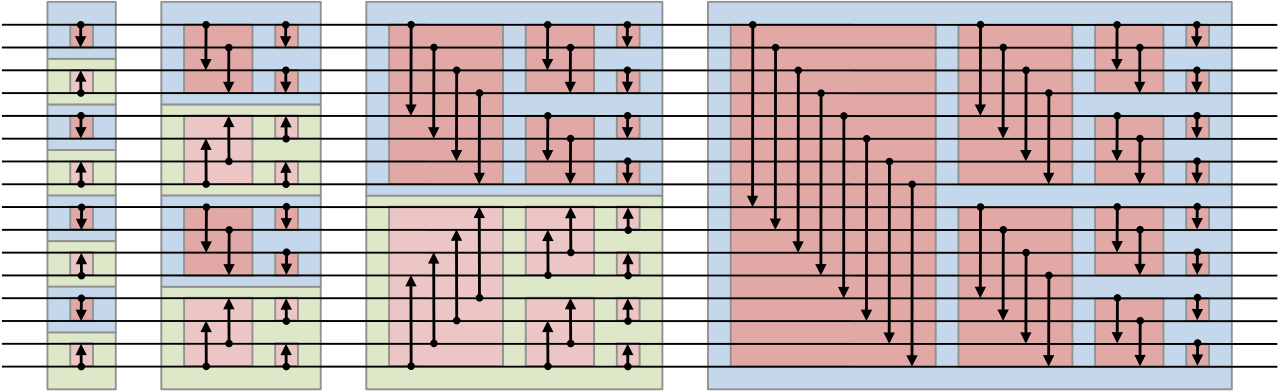
\includegraphics[width=5in]{fig/1280px-BitonicSort1.svg.png}
    \caption{双调排序的流程图\cite{bitonic_wiki}}
    \label{fig:bitonic}
\end{figure}

如图\ref{fig:bitonic}所示,双调排序是一个高度并行的算法,如果串行运行,其时间复杂度为$\mathcal{O}(n\log_{2}{n})$,而当有$\frac{n}{2}$个可用线程时,则其时间复杂度为$\mathcal{O}(\log_{2}{n})$。\cite{bitonic_wiki}


% \begin{breakablealgorithm} 
%   \caption{初始化obj文件信息——对应MeshSimplify类中readfile函数,Face类calMatrix函数} 
%   \begin{algorithmic}[1] %每行显示行号  
%       \Require obj文件,顶点、边、面列表
%       \Ensure 是否读取成功
%       \Function {calMatrix}{$Face$}  
%               \State $normal \gets e1×e2$  
%               \State $normal \gets normal/normal.length$
%               \State $temp[] \gets {normal.x, normal.y, normal.z, normal· Face.v1}$
%               \State $Matrix[i][j]=temp[i] * temp[j]$ 
%               \State \Return{$Matrix$}  
%       \EndFunction
%       \State 根据obj的v和f区分点面信息,读取并加入列表
%       \State $scale \gets $记录点坐标中距离原点最远的分量,以便后续OpenGL进行显示
%       \State $ori \gets $记录中心点,便于OpenGL显示在中心位置,避免有的obj偏移原点较多
%       \State 根据三角面片信息,计算一个面的三条边
%       \State 计算每个面的矩阵$\gets calMatrix$
%       \State 将每个面的矩阵加到各点,由点维护\\
%       \Return True
%   \end{algorithmic}  
% \end{breakablealgorithm}

% 代码
% \begin{lstlisting}[title=逐列访问平凡算法,frame=trbl,language={C++}]
%     int main(int argc, char* argv[]) {
%     	int myid, numprocs;
%         memset(metric, 0, sizeof(float)*D*T);
%         memset(query, 0, sizeof(float)*Q*T);
%     	MPI_Init(&argc, &argv);
%     	MPI_Comm_rank(MPI_COMM_WORLD, &myid);
%     	MPI_Comm_size(MPI_COMM_WORLD, &numprocs);
%     }
% \end{lstlisting}


%——————————————————————————————————————

\subsection{矩阵乘法}

除了充分利用GPU之外,针对异构并行计算机编写的程序也需要考虑对各种架构进行充分地利用。在上文中提到的超算中,虽然GPU或协处理器提供了大部分的双精度浮点性能,但如果仅仅只将CPU作为GPU的控制器,所浪费的CPU性能也是非常多的。
~
\begin{figure}[!htbp]
    \centering
    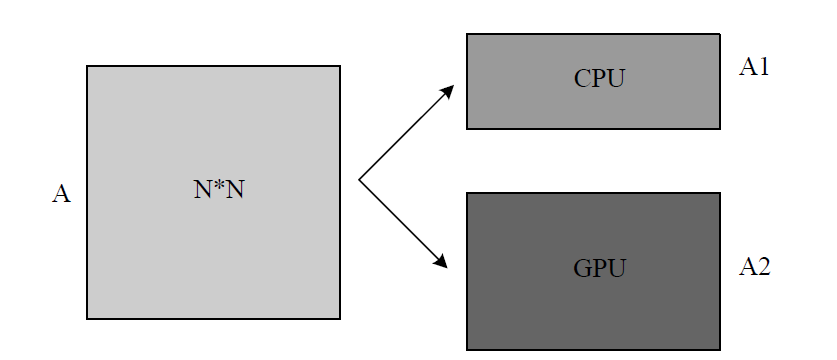
\includegraphics[width=3in]{fig/matrix_divide.png}
    \caption{通过预先的性能测量,确定矩阵分割的比例\cite{gpu_martix}}
    \label{fig:matrix_divide}
\end{figure}

对于这种情况,可以通过性能分析,确定CPU和GPU求解问题效率的比值,并根据这个比值进行任务调度。比如,两个$N\cdot N$的矩阵$A, B$相乘,我们就可以将矩阵$A$按比例上下分割开来,形成矩阵$A_{1}$和$A_{2}$,$A_{1}$在CPU和$B$进行点乘运算,$A_{2}$则和$B$一起发送给GPU进行点乘,这样既节省了数据在总线上的传输时间,也充分利用了CPU的性能。\cite{gpu_martix}

~


值得留意的是,最近几年,TOP500登顶的两台计算机——神威太湖之光和富岳又回到了单芯片的路线,也就是说这些超算的节点中,已经不再是CPU+协处理器或CPU+GPU这样有多种处理器的配置了。但是这些超算仍然是异构的——神威太湖之光所使用的神威26010处理器在片上集成了融合异构众核架构、单芯片具有4个运算控制核心和256个运算核心;而富岳所使用的A64FX也是48个计算核心、4个辅助核心的异构结构。总而言之,单芯片超算是对异构并行计算架构的一种肯定与发展。\cite{sw26010}\cite{a64fx}

% 参考文献\cite{adams1995hitchhiker}\cite{shin2016deep}
    
% 多行公式
% \begin{align}
%   a+b = a + b \\
%   \frac{a+b}{a-b}
% \end{align}

% 行内公式:$\sum^N_{i=1}$

% \textbf{超链接}  \href{http://youtube.com/}{YouTube}

% 带标号枚举
% \begin{enumerate}
%   \item 1
%   \item 2
% \end{enumerate}

% 不带标号枚举
% \begin{itemize}
%   \item 1
%   \item 2
% \end{itemize}

%\xiaosi{切换字体大小}

%----------------------------------------------------------------
\section{以能效为目标的异构并行计算机}
\subsection{ARM}
作为在便携设备上得到广泛应用的架构,ARM架构的功耗控制极为优秀,而近年来智能手机市场的蓬勃发展,对arm架构的性能和效率提出了更高的要求。为了满足这样的要求,ARM公司于分别于2011年和2017年推出了异构多核的结构配置方案——big.LITTLE和其升级版DynamIQ。

\begin{figure}[htbp]
\centering
\subfigure[ARM big.LITTLE架构]{
\begin{minipage}[t]{0.48\linewidth}
\centering
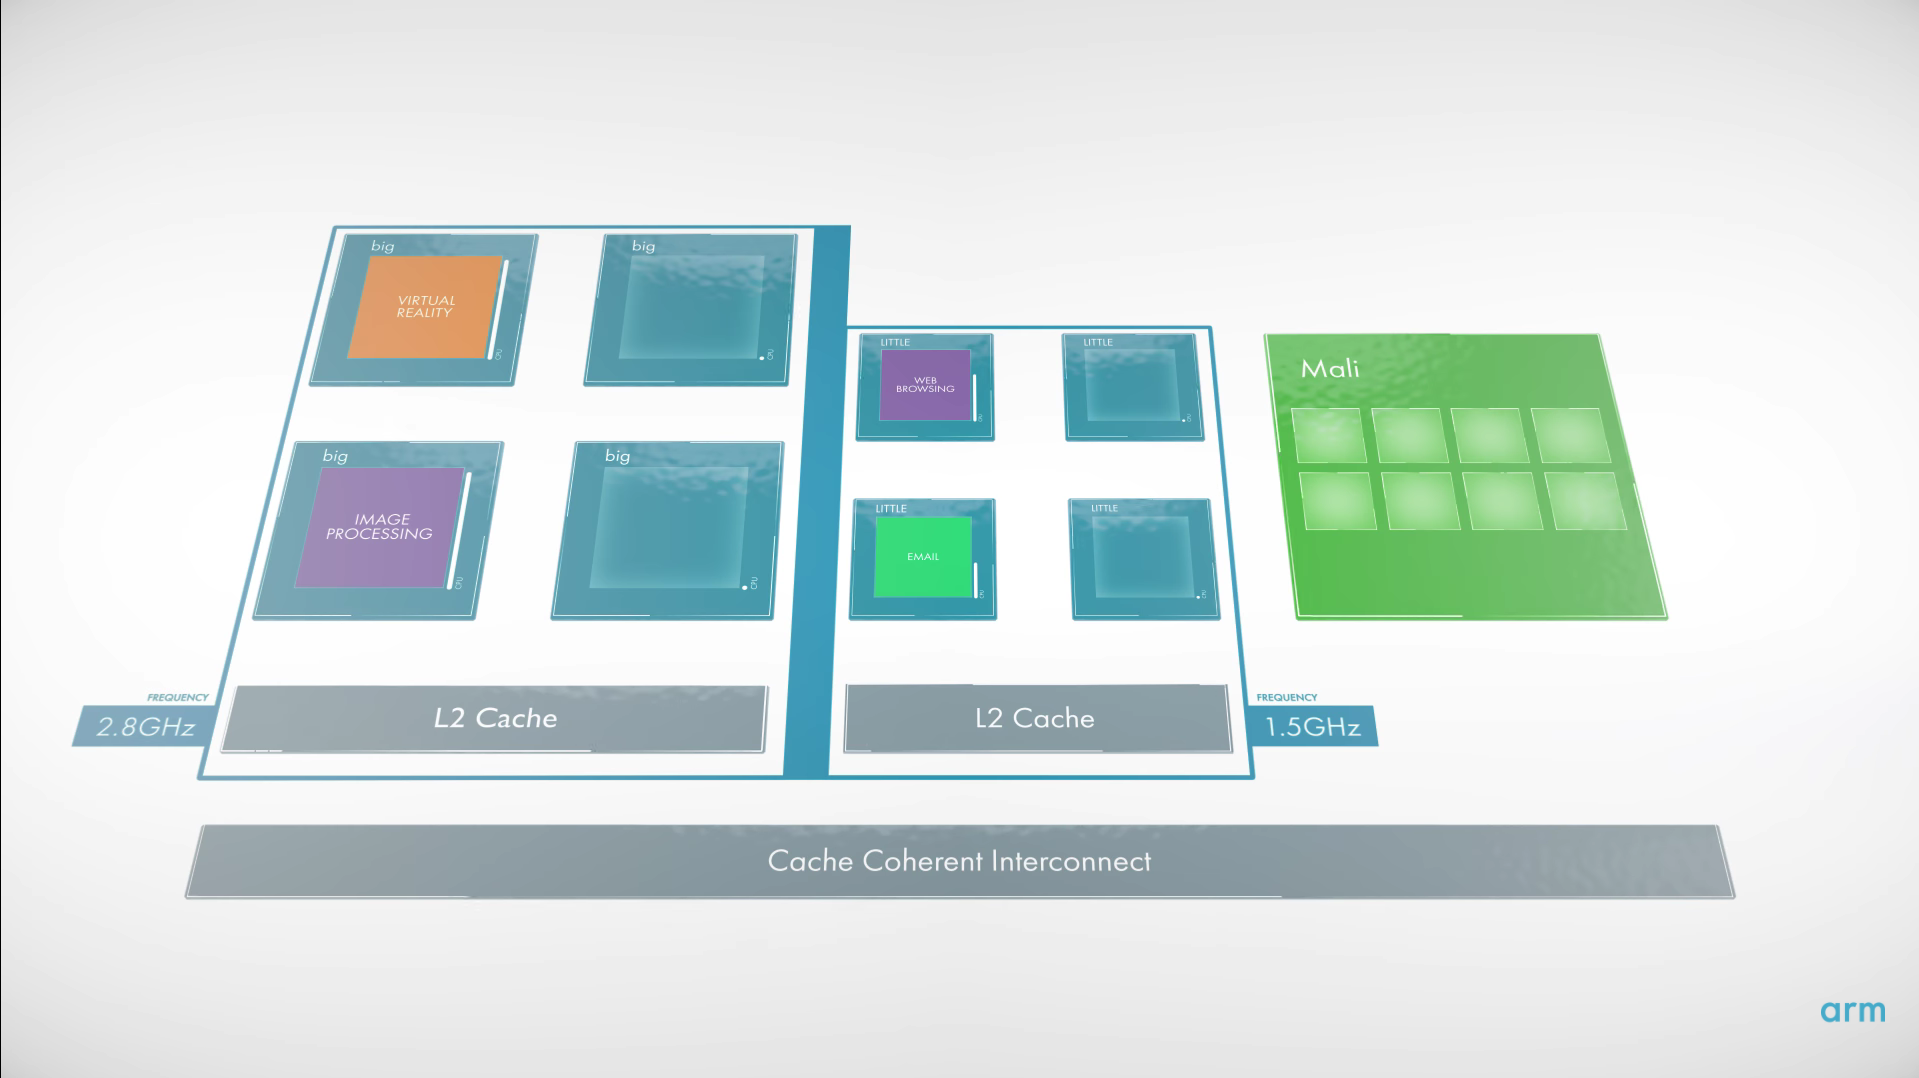
\includegraphics[width=2.8in]{fig/ARM_BIG_LITTLE.png}
\end{minipage}%
}%
\subfigure[ARM DynamIQ架构]{
\begin{minipage}[t]{0.48\linewidth}
\centering
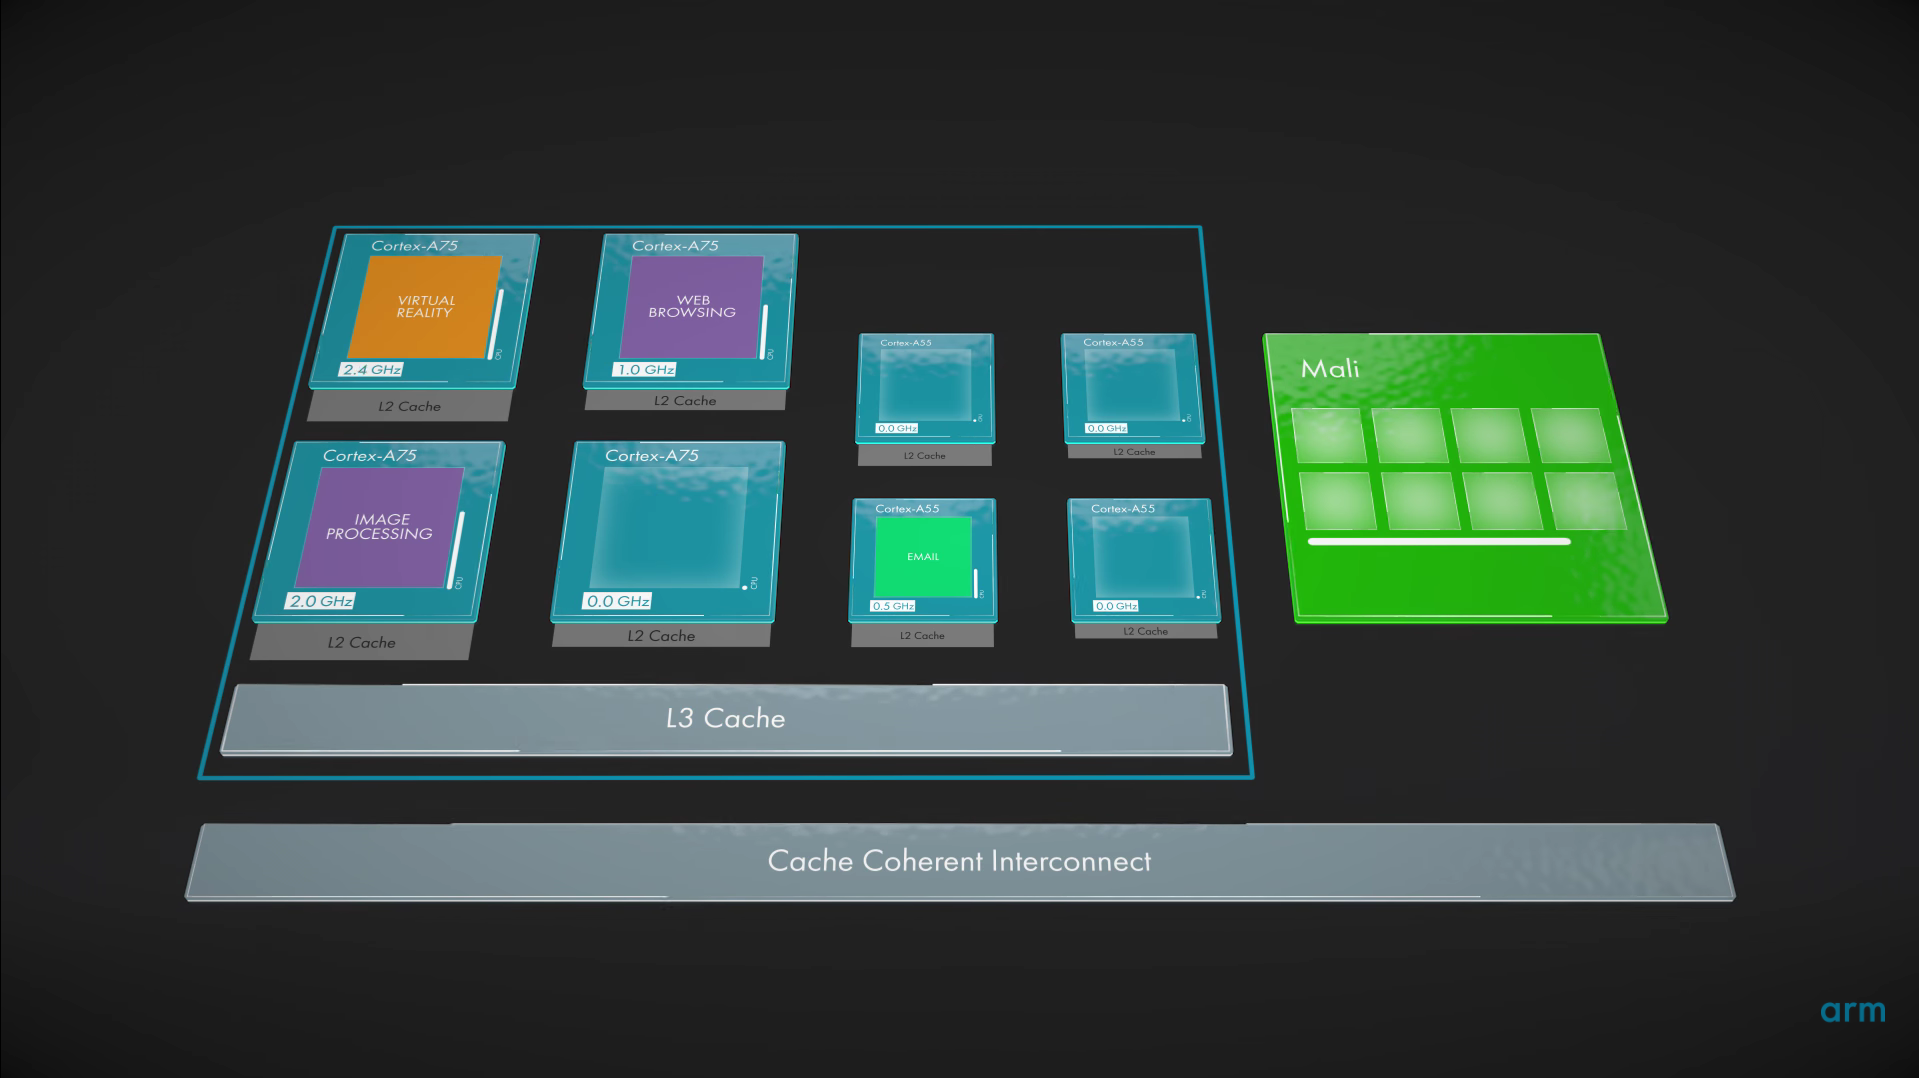
\includegraphics[width=2.8in]{fig/ARM_DYNAMIQ.png}
\end{minipage}%
}
\centering
\caption{ARM公司推出的两种异构多核配置\cite{arm_dynamiq}}
\label{fig:arm_heter_cores}
\end{figure}

DynamIQ相较于big.LITTLE,最大的优点就是新增了可以更自由配置的大小核心数量的特性。在big.LITTLE中,相同的核心被打包在同一个集群(Cluster)里,一种典型应用是,四个大核(Cortex-A15)和四个小核(Cortex-A7)被分别打包为两个集群(Cluster),而两个集群之间则通过一致性互联总线(Coherent Interconnect)链接。而到了DynamIQ中,单个集群中核心的数量变为了8个,且不同的核心可以被打包在一个集群里。这样一来,购买ARM IP的客户便可以根据自己的需求自行配置大小核的比例 \cite{arm_dynamiq}

大小核的架构也对软件的设计提出了更高的要求。操作系统需要了解当前的电量状态,每个线程的性能需求等信息,并根据这些信息将线程转移到适合它们的核心上去,只有合理的调度算法,才能发挥大小核架构在效率方面的潜能。

\subsection{X86}

随着近年来笔记本电脑市场的扩张,在PC市场具有支配性地位的X86处理器设计公司们也愈来愈需要关注其产品能耗比这项指标了。英特尔公司在其最新发布的Alder Lake架构中,也使用了异构多核的技术。Alder Lake具有两种核心——被称为Golden Cove的性能核心,以及被称为Gracemont的效率核心。英特尔简化了效率核心的设计————四个效率核心的面积才相当于一个性能核心的面积,其具有“深前端”(64KB的大容量指令缓存、更准确的分支预测)、“广后端”(256个乱序执行窗口、17个执行端口)的设计特点,再配合最新的Intel 7制造工艺,效率核心获得了极好的能效比,面积较小的核心也降低了总线的长度,带来了更高的访存性能。而性能核心除了具有更大的256KB指令缓存和更复杂的乱序执行模块之外,还为了人工智能相关计算新增了矩阵乘法引擎。\cite{intel_archi_day}\cite{intel_alder_lake}

\begin{figure}[htbp]
\centering
\subfigure[效率核心Gracemont]{
\begin{minipage}[t]{0.48\linewidth}
\centering
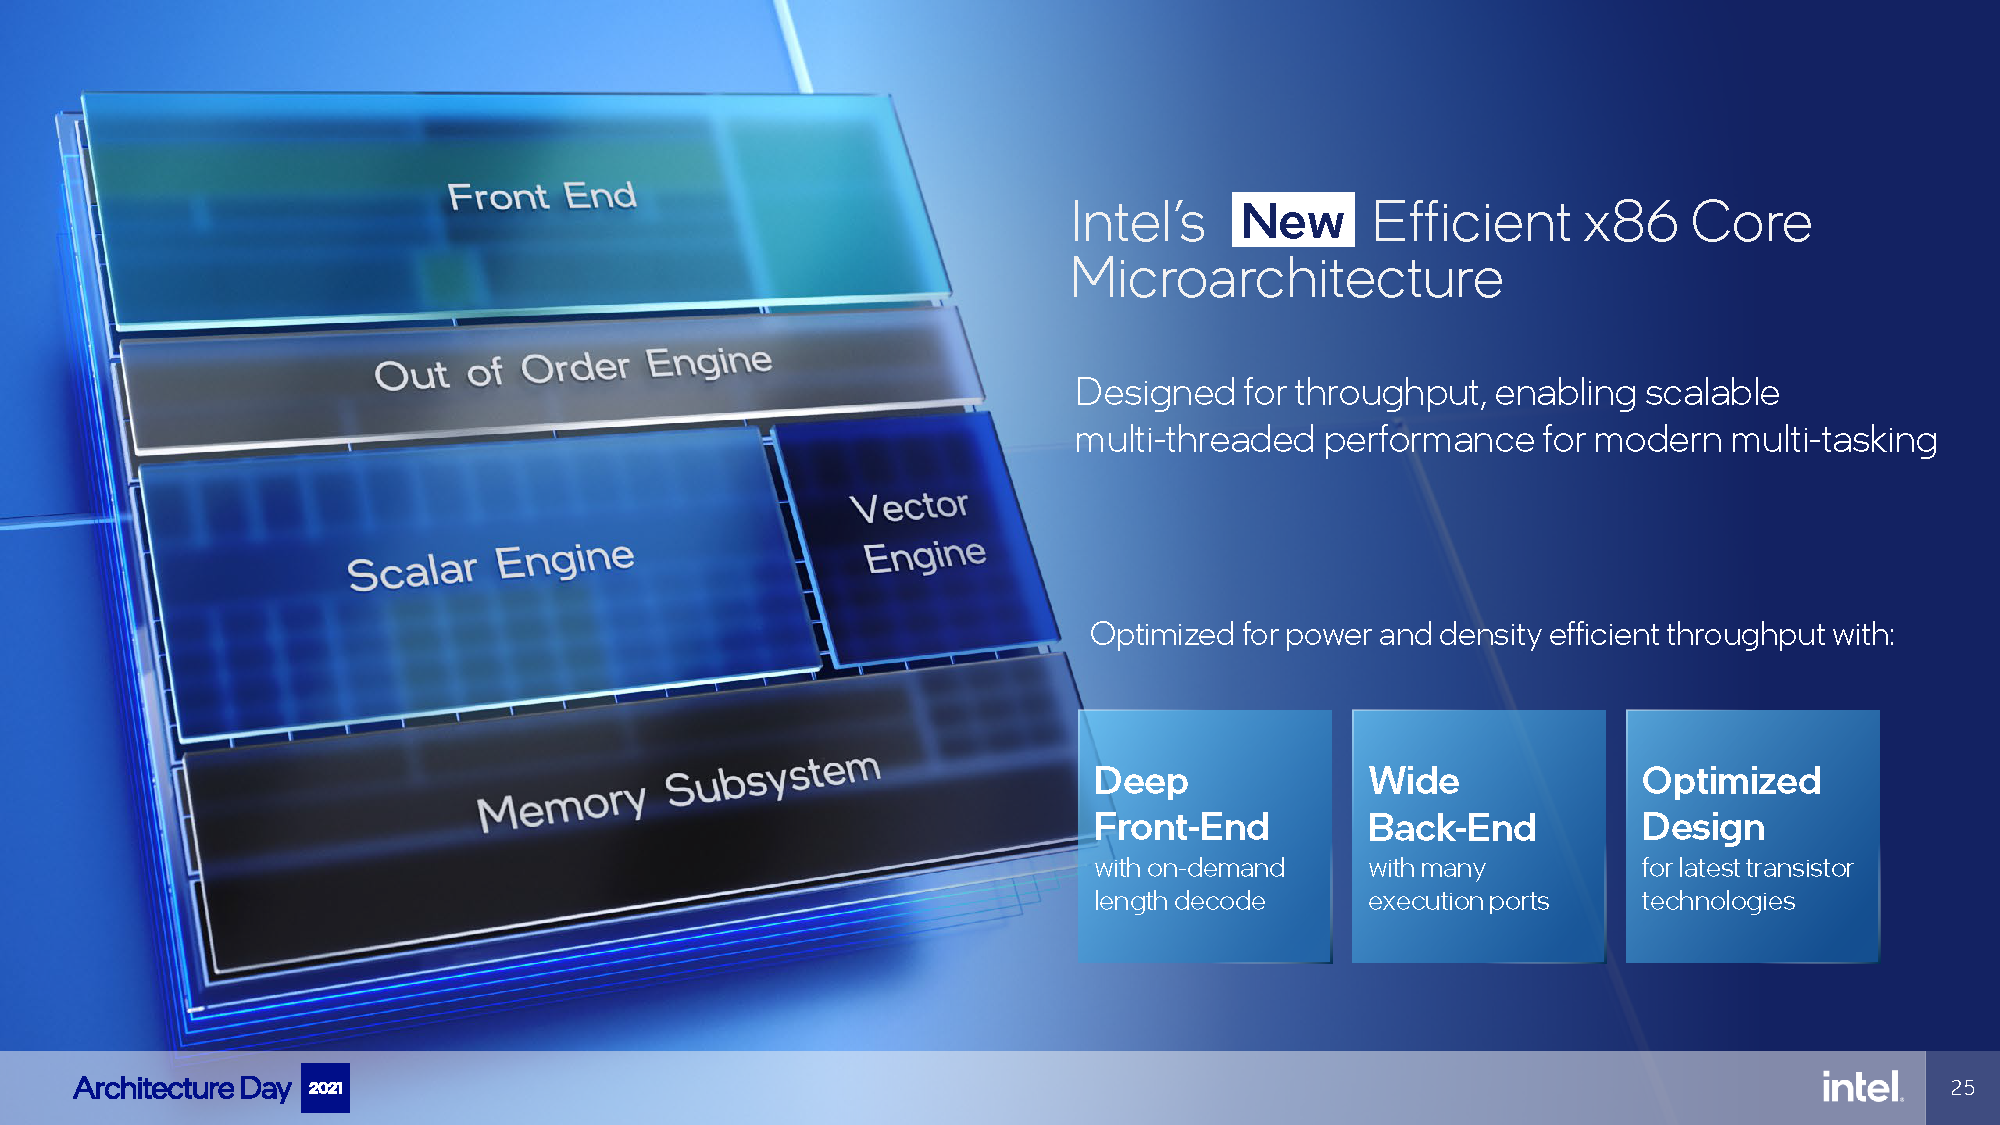
\includegraphics[width=2.8in]{fig/alderlake_e_core.png}
\end{minipage}%
}%
\subfigure[性能核心Golden Cove]{
\begin{minipage}[t]{0.48\linewidth}
\centering
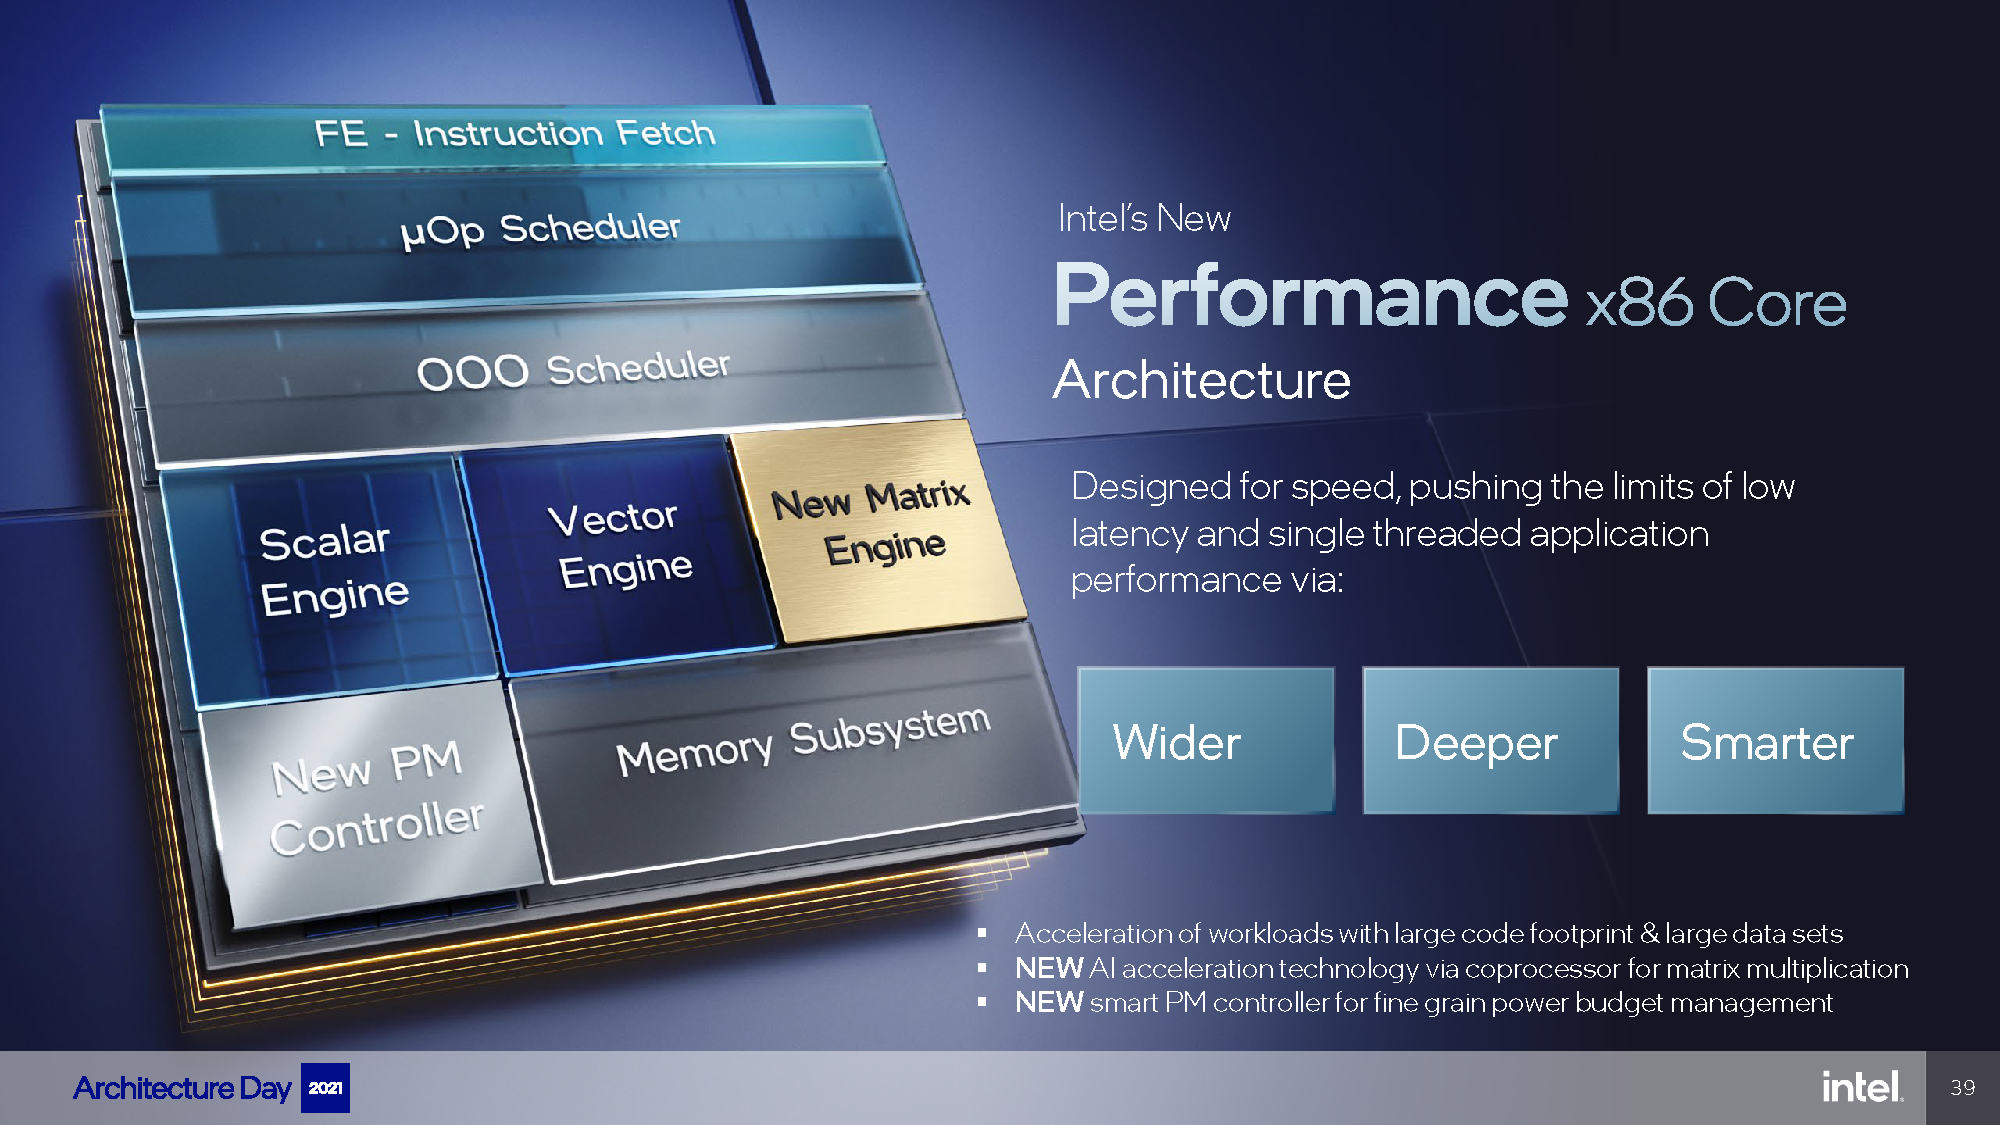
\includegraphics[width=2.8in]{fig/alderlake_p_core.png}
\end{minipage}%
}
\centering
\caption{Alder Lake架构中的两种核心\cite{intel_archi_day}}
\label{fig:intel_alderlake}
\end{figure}

英特尔Alder Lake也有配套的调度技术——Thread Director。当一个任务需要较少的性能时,Thread Director会将其优先分配到效率核心上,反之,则会被分配到性能核心上。而当所有的性能核心都被占用时,出现了一个需要更高性能的任务,比如说需要性能核心矩阵处理性能的AI任务,Thread Director便会向操作系统建议,将一个在性能核心上运行的任务转移到效率核心上。此外,如果性能核心上出现了等待状态的线程,它也会被移动到效率核心上运行。Thread Director这项技术可以使得处理器在各种不同的使用场景下做到性能与功耗的平衡。\cite{intel_alder_lake}


%----------------------------------------------------------------
\section{总结}
异构计算机在提升超级计算机性能、帮助移动设备获得更好的能效比这两件事上已经表现出了其巨大的潜力。我们应该相信,随着相关软硬件技术的发展,异构计算机将会变得更快、更强、更环保。
%----------------------------------------------------------------
\newpage
\bibliographystyle{plain}
\bibliography{references} 
\end{document}
